%\documentclass[10pt,a4paper,final,oneside,openany,article]{memoir}
%\documentclass[letterpaper,a4paper,10pt]{article}
\documentclass[10pt,letterpaper,two column,final]{article}
\usepackage[utf8]{inputenc}
\usepackage[british]{babel}
\usepackage{hyperref}
\setcounter{tocdepth}{3}
%\usepackage[draft]{fixme}
\usepackage{abstract}
\usepackage{todonotes}
\usepackage{longtable}
\usepackage{amsmath}
\usepackage{pifont}
\usepackage[small, bf]{caption}
\usepackage{algorithm}
\usepackage{algorithmic}

%% FONT
%\usepackage[T1]{fontenc}
%\usepackage{lmodern}
%\usepackage[urw-garamond]{mathdesign}
% Fonts configuration
%  - Palatino and Bitstream Vera Sans Mono for verbatim
\usepackage[T1]{fontenc}
\usepackage{palatino}
\usepackage[sc]{mathpazo} % Math font for Palatino
\usepackage{bera}
\linespread{1.05} % Palatino needs more leading (space between lines)
\usepackage{microtype}
\usepackage{graphicx} % ++
\usepackage{color}
\definecolor{kugrey}{rgb}{.4,.4,.4}
\usepackage{listings}
\usepackage{amssymb}
\lstset{ %
    language=Python,                % choose the language of the code
    frame=single,                   % adds a frame around the code
    keywordstyle = \footnotesize\ttfamily,
    commentstyle = \color{kugrey}\textit,
    stringstyle = \ttfamily,
    basicstyle   = \footnotesize\ttfamily,
    numberstyle=\tiny,
    sensitive = true,
}

%% odds and ends
%\chapterstyle{hangnum}
\setcounter{secnumdepth}{2}

%HEADINGS
\title{Constructing Models For Diagnosing Rare Diseases}

\author{Brian S. Mathiasen $-$ soborg@diku.dk \\
        Henrik G. Jensen $-$ henne@diku.dk\\
        \small{Supervisor: Jakob Grue Simonsen $-$ simonsen@diku.dk} \\
        \\
        Department of Computer Science\\
        University of Copenhagen\\
        Universitetsparken 1\\
        DK-2100 Copenhagen, Denmark
}

\date{\today} %\today

%%
\begin{document}
\maketitle
%\listoffixmes
%\tableofcontents


\begin{abstract}
In this paper we design and construct models for assisting physicians
with the task of diagnosing rare diseases. Using a prior knowledge of
rare diseases consisting of \textit{disease name} and \textit{abstract},
we utilize the \textit{Google Search Engine} to harvest additional
knowledge of 3882 rare diseases to expand the model. Using various
techniques, ranging from data set noise reduction, to Machine
Learning and Natural Language Processing are applied in order to
construct different models and subsequently compare them in terms of
prediction precision.

\paragraph{Results: }The most successful approach (Orphanet Abstracts+Noise Reduced googled
data with TFIDF modelling) places 86\% (37 out of 43) of the diseases
within the top 5 predicted results and 95\% (41 out of 43) within top
20. The model is based on harvested information and prior information
(abstracts from Orphanet), and is implemented using a basic \textit{Term
Frequency - Inverse Document Frequency} model.
\end{abstract}
%%-----------------------------
%\newpage

\section{Preface}
\subsection{Expectations to the reader}
The reader is expected to have knowledge in Computer Science at a
Master's degree entry level.

It is expected that the reader has read the project
\cite{jensenandersen}.

We expect the reader to have knowledge of Natural Language Processing (NLP)
techniques, in particular POS-tagging and phrase chunking. It is also
required to have knowledge of the foundations and overall methodology of
Machine Learning.

\subsection{Source code and package dependencies}
The source code, this report and the previous project by
\cite{jensenandersen} is available at the repository:
\url{http://code.google.com/p/disease-crawler/}
%Installation and usage is exclusively the responsibility of the user.
The system is developed in Python version 2.6.6 on Ubuntu 10.10,
utilizing the following external modules:
\begin{itemize}
\item nltk \footnote{\url{http://nltk.org}}, Ubuntu repository module: \texttt{python-nltk}
\item numpy \footnote{\url{http://numpy.scipy.org}}, Ubuntu repository module: \texttt{python-numpy}
\item hcluster \footnote{\url{http://code.google.com/p/scipy-cluster/}}
\item lxml \footnote{\url{http://lxml.de}}, Ubuntu repository module: \texttt{python-lxml}
\item sqlite3, Ubuntu repository module: \texttt{python-sqlite}
\end{itemize}

The full test descriptions along with search queries are likewise
available at the above mentioned repository. The results for the tests
are available in the appendices.

%\subsection{How-to}
%\paragraph{Building a model: }

%\paragraph{Querying a model: }

%\paragraph{Interpreting the result: }


\section{Introduction}
%\label{chap:introduction}
Physicians have expressed a need for aiding in the process of diagnosing
rare diseases \cite{googlingdiagnosis}, and point towards using the
Internet as a resource for information gathering, with particular focus
on utilizing Google or other popular search engines
\cite{googlechangemedicine} \cite{diagnosissearchengines}.

%The current process of automating this process relies heavily on static
%information, which is only expanded through manual interaction. \fxwarning{citation needed}
%\url{http://www.wrongdiagnosis.com/},
%\url{http://www.rarediseases.org/}, \url{http://www.orpha.net/}.

In this project, we investigate several methods for automating
information collection of specific features from rare diseases. The
project is mainly developing proof of concept models, on which a
practising physician can query a case report or a number of search terms
and get a list of disease predictions based on the knowledge of the
model.

The basic model is constructed given information of 3882 diseases\footnote{We have chosen not to discriminate between diseases groups of
diseases.}, with corresponding abstract or disease group information.
This information, together with the disease name and other relevant
terms are used to harvest the Internet for related information to expand
the knowledge of that particular disease.

A number of post-processing techniques are now applied to the basic
model to develop the final proof-of-concept models, based on different
characteristics and processing strategies.

% The models are sketched as
%follows:
%\begin{description}
%\item[Unigram] This model is similar to the model developed in the proje
%\item[Cleansed Model]
%\item[Unigram+NLP]
%\item[ICD10 model]
%\end{description}


%In order to increase the prediction precision, the model is expanded by
%harvesting information of some disease through a number of iterations on
%popular search engines. The harvested data is sanitised and irrelevant
%or low-information paragraphs are removed to reduce noise within the
%model. The prediction process is performed by, given a query, a number
%of diseases are returned that match the the query, in addition to
%ICD10\footnote{The International Statistical Classification of Diseases
%and Related Health Problems 10th iteration (ICD10) is a classification
%of diseases, signs and symptoms, classified by the World Health
%Organization (WHO).} code clusters and Natural Language Processing (NLP)
%based models. \todo[inline]{rewrite to make it crystal clear!}


%We use Natural Language Processing (NLP)
%provided through a Python library \cite{NLTK} to extract unique
%information from some description of the disease, and use Machine
%Learning to refine the search within the model.

%by assuming certain semantic and
%syntactic properties of symptoms and medically related phrases and
%terms.


\subsection{Limitations}
We have not developed a fully automated system that with a simple
interface is able to take a query and return a prediction. The system
and models are developed as autonomous modules and have not yet been
fine-tuned or assembled as a complete program.


\subsection{Content outline of this document}
In section \ref{chap:previouswork} we will outline current and previous
work and briefly discuss their respective approaches to solving the
problem.

In section \ref{chap:method} we will present an overview of the methods
used, and go into detail with the most important steps, by discussing
information harvesting, feature extraction, modelling and prediction.

% of each of
%the developed models.

In section \ref{chap:implementation} we will go into the implementation
details of the various models, discuss unique traits and clarify which
methods are employed in each model.

%highlighting the overall architecture and
%pipeline of constructing the models, and clarify which methods are used
%in each model.

% while
%explaining the more important parts of the architecture.

In section \ref{chap:test} we present the results from our experiments,
here among blind tests, BMJ and Orphanet. We will discuss the results
based on statistical significance and descriptive analyses.

Finally, in section \ref{chap:conclusion} we will conclude the project,
highlight the most important test results and discuss major implications
and advantages of the system, methods and tests. We will finally propose
a number of topics for future work.


%In the following we will present and highlight current and previous work
%within this domain. In chapter 3, we will discuss our method
%methodically, with particular focus on construction of model and feature
%extraction and post processing of harvested information.
%Then we will explain how we tested the system and argue statistical
%significances by comparing to previous work, as well as assessing the
%viability of our system as it is.
%Finally we will conclude our paper and discuss implications and other
%thoughts relevant to our method, while also proposing a number of topics
%for future work.

\section{Previous Work}
\label{chap:previouswork}
The article \cite{googlingdiagnosis} assesses the viability of using
Google as a diagnosis aid, despite the tests being done manually with
little consideration with regard to automation or test reliability and
validity. Their method yield a correct diagnosis in 15 (58\%, 95\%
confidence interval 38\% to 77\%) cases.


\cite{jensenandersen} proposed a system for diagnosing rare diseases
using vector space models and text mining. They showed a potential in
automating such a process, but their results were not statistically
significant. Their system did not rely on prior knowledge of particular
diseases, but still showed that around 60\% of the tests were
satisfactory \footnote{The criterion is that the correct disease located
within the top 20 predictions.}.

Our colleagues Radu Dragusin and Paula Petku from the department of
Computer Science at Copenhagen University investigate a related way of
automating information gathering to what we are presenting. However, as
this is a work in progress, we do not have access to further information
at this point in time \cite{radupaula}.



%Our system will move on to the next step and introduce intelligent
%automation through a number of predefined criteria and utilizing several
%machine learning and natural language processing techniques.


%The editorials \cite{googlechangemedicine} and
%\cite{diagnosissearchengines} suggest Google and search engines in
%general as being a very strong player in the task To perform the initial
%testing we mimicked the previous project where a TF-IDF\footnote{Term Frequence - Inverse Document Frequence.} matrix was build
%using information (abstracts,titles, keywords) gathered form Pubmed. The
%knowledge of search engines being a valuable source of information is
%apparent, but the shear amount of misinformation and noise from regular
%searches make such a method in it’s current incarnation unreliable and
%error prone.\fxwarning{citation needed} \todo[inline]{Omformuler,
%præciser!}


%(Our goal is to refine and provide means for filtering out this noise
%and focus on harvesting information from related material with reference
%to the original search terms as well as specific criteria for the text
%mining process.)


%Inspiration for a system: Online Search Engine specialised for
%diagnosing stuff etc.
%http://www.healthline.com/symptomsearch

%This system is based on simple searches that relies on an already
%established database of diseases with appropriate meta-information. The
%user is able to search for symptoms and can narrow down the search by
%adding several symptoms. The system will then present a list of possible
%diseases according to some relevance criterion.

%(It is an end-user focused system, while our system will be a back-bone
%focused system, attempting to establish a model on which queries may be
%imposed. It will as such automate the information collection based on
%several machine learning and natural language processing techniques
%appropriate for the needs.)


%Google Health: http://www.google.com/intl/en-US/health/about/index.html


%Article by practising doctor on “do’s and don’t’s when using Google as
%diagnosis aid”:
%http://vitualis.wordpress.com/2007/02/26/google-based-medicine/


\section{Method}
\label{chap:method}
In the following, the methods used to compute the various models will be
explained at a high abstraction level. We will highlight the basic model
used to compute unigram models, similar to that presented in
\cite{jensenandersen}, present the use of Natural Language Processing
techniques to allow extracting specific knowledge to build an NLP based
model or tailored N-gram model. Finally we will highlight the use of
ICD10 codes to categorise related diseases.

The application of and concrete implementation specific details of the
final models will be explained in section \ref{chap:implementation}.


\subsection{General Procedure}
To get an overview of how to build any model, the general procedure will
be explained in this section.
Ultimately, the needed tools for building the model are
\begin{description}
\item[data set] we utilize data (disease name, abstract/description)
acquired from Orphanet.
\item[mathematical model] We will use the TF-IDF model as a basis, and
from this offset develop specific methods to improve the results.
\end{description}

Additionally, we look into using an information gatherer to expand the
knowledge of the given data set. Using the Google Search engine allows
us to harvest information from a large range of websites with reasonable
ease.


%To establish a foundation for expanding the knowledge of rare diseases
%the data received from Orphanet, an online database of information
%specialised on rare diseases, is initially used as prior knowledge to
%harvest additional information from the Internet.

%As one of the premises of the project was to introduce prior knowledge
%of the disease model, we needed to process our available data. We were
%given a large corpus of data from Orphanet \ref{app:orphanet},
%consisting of \texttt{\{orphanum, disease name, disease
%description/abstract, maybe author and date\}} for each disease in the
%data set.\todo[inline]{Rewrite this nonsense.}

The data is processed similar to what is described in
\cite{jensenandersen}, and will thus be used to bootstrap the knowledge
of each disease, allowing us to iterate and harvest additional
information using various harvesting techniques roughly covering the use
of the \textit{Google} search engine to collect an array of websites
given a query relevant to the disease (disease name and a possibly a
number of keywords). For each website, we will collect paragraphs given some acceptance threshold and
save it for further processing.

%For each
%accepted paragraph we use NLP to identify candidates for relevant terms
%and phrases that will then be used to expand the model. 

The abstract flow model is shown in figure \ref{fig:flow}. The data set
is processed (cleansed for noise, stemmed, NLP, etc.) and fed into the modelling
procedure (TF-IDF or similar). The model is then expanded using various
searching strategies, in this case using Google, where the data set is
feature extracted, processed, and fed into a new modelling procedure.
This iterative approach is initiated until a reasonable amount of data
is collected. In this project, only one iteration of using the Google
search engine per disease is executed.

\begin{figure}[htp!]
\begin{center}
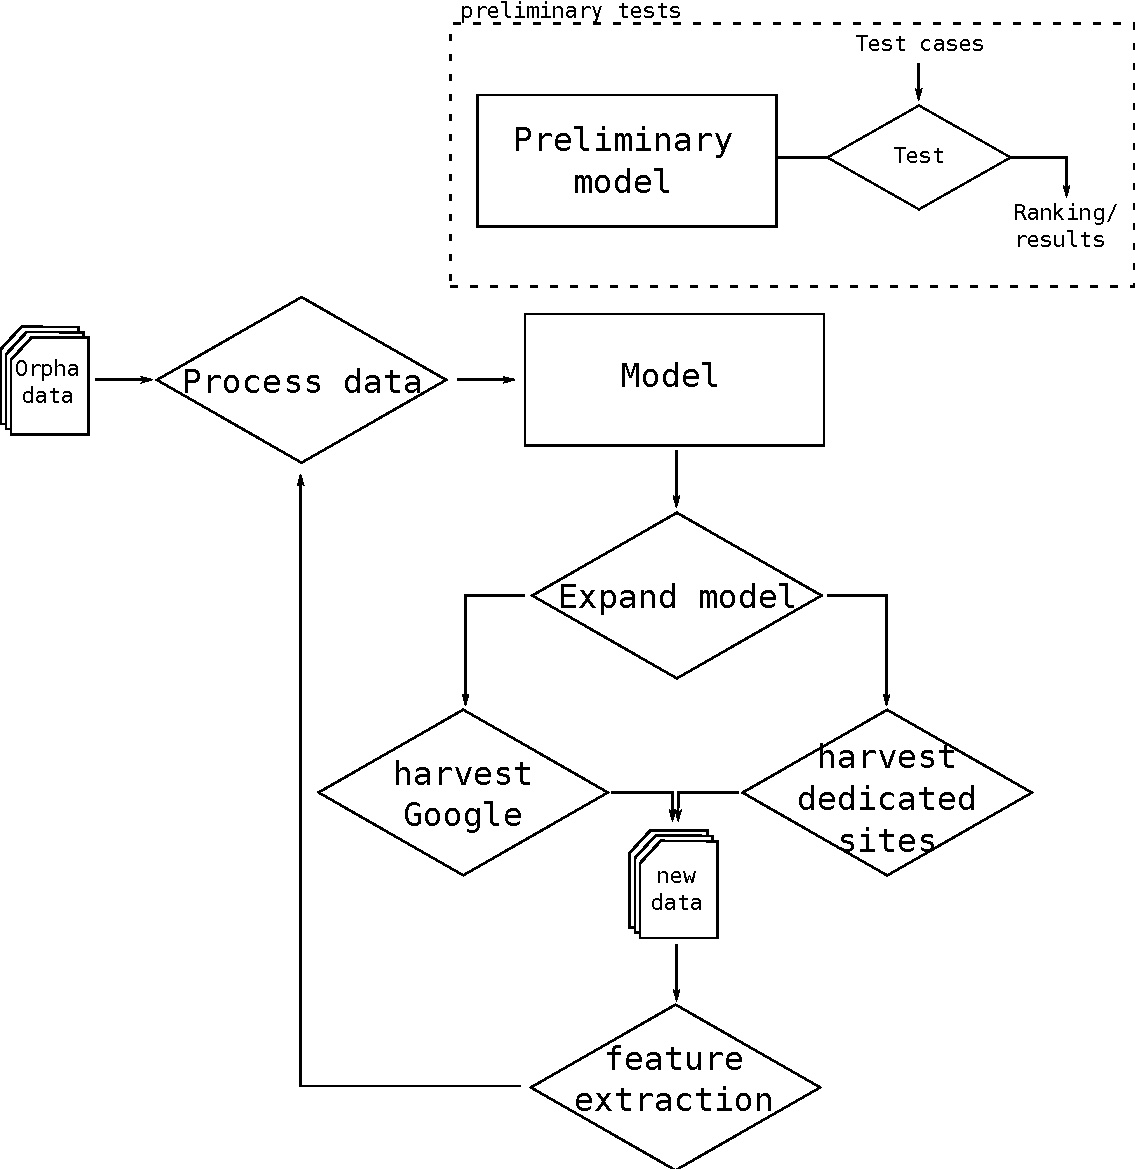
\includegraphics[scale=0.4]{images/pipeline}
\caption{Systems diagram.}
\label{fig:flow}
\end{center}
\end{figure}

%[As several individual models are being constructed, we will highlight
%the most important cornerstones of all the methods used independently
%across all the models.
%We initialise by explaining how the basic model is constructed and how
%we have refined it into a number of proof of concept models.]
%\todo[inline]{rewrite previous to make sense and put it in context}

%\todo[inline]{Something N-gram machine learning here.}

\subsection{Building the TF-IDF model}
\label{chap:basicmodel}
The TF-IDF model is built using the prior information available
from Orphanet. The models in this project are at an abstract level
identical to the model constructed in \cite{jensenandersen}. While
\cite{jensenandersen} used information gathered by automatically
searching the Pubmed online database
\footnote{\url{http://www.ncbi.nlm.nih.gov/pubmed/}}, prone to contain
irrelevant information, we use validated abstracts provided by Orphanet,
data gathered by using Google and subsequently filtered with various
NLP techniques.


%To perform the initial testing we mimicked the setup of
%\cite{jensenandersen} where a TF-IDF matrix was build using information
%(abstracts,titles, keywords) gathered form Pubmed.

%A sparse term-disease matrix (similar to the well-known term-document
%model) is built over the abstracts received from Orphanet.
Each row in the matrix, representing the model, is a feature vector of a
disease with the features being a list of term frequencies. Prior to the
creation of the matrix, the terms are stemmed (using the Porter stemming
algorithm \cite{porterstemming}) and stopwords \footnote{The stopwords
are defined by a list of 127 English words provided by the Python NLTK
library (\texttt{nltk.corpus.stopwords.words("english")}} along with
non-alphanumerical\footnote{Characters that do not contain the value of
a number or a letter.} symbols are removed.

Stemming a word involves reducing it to its most basic form or root,
removing morphological and inflectional endings from the words. E.g.
walking, walker, walks have the affixes \textit{-ing}, \textit{-er} and
\textit{-s}, with the common root \textit{walk}.


The term-disease matrix is then processed using the
TF-IDF model (as originally proposed by \cite{tfidf}) along with
additional logarithmic smoothing of the $tf_{t,d}$-parameter to flatten
term-burstiness (\cite{burstiness}).

The TF-IDF model is thus constructed as following:
\[
w_{t,d} = log(tf_{t,d}+1)\cdot log\frac{|D|}{|\{d'\in D|t\in d'\}|}
\]
where $tf_{t,d}$ is term frequency of term $t$ in disease $d$, $|D|$ 
the total number of diseases in the disease set, and $|\{d'\in D|t\in
d'\}|$ the number of diseases containing the term $t$.

To compare the precision of the new model to the old model in
\cite{jensenandersen}, we applied the same test queries (search terms)
to the model using the same scoring-scheme to obtain a rank for each
disease. The rank of each disease can be interpreted as being the
precision of the model.

When a query is given, it is stemmed and stopwords are removed. Each
disease-vector that contain one or more of the queried terms is given a
score which is based on a summation of each of the weights of the
queried terms relevant to the disease.
\[
s_{d} = \displaystyle\sum\limits_{t_1}^{t_n} w_{t,d}\quad t \in Q
\]

\paragraph{Example}
Consider four diseases, each consisting of up to three terms,
\{headache, pain, insomnia\}:
\begin{align*}
d_{0} &= \{insomnia\} \\
d_{1} &= \{headache, insomnia \} \\
d_{2} &= \{insomnia \} \\
d_{3} &= \{headache, pain, insomnia\}
\end{align*}

Then the TF-IDF matrix is constructed, at this point ignoring the
logarithmic smoothing:

\[ w = \left| \begin{array}{ccc}
0 & 0 & 0.25 \\
0.5 & 0 & 0.25 \\
0 & 0 & 0.25 \\
0.5 & 1 & 0.25  \end{array} \right|.
\]

In this case the queried terms correspond with all the terms of
$w$, i.e. $Q = \{headache, pain, insomnia\}$, then the summation of the
weights of the queries terms are given as

\[ s = \left| \begin{array}{c}
0.25 \\
0.75 \\
0.25 \\
1.75 \end{array} \right|.
\]
Thus the bottom entry, disease number 3 (zero-indexed), with a score of
$1.75$ is the model's prediction of the correct disease/diagnosis.
\ding{111}\newline

%Though the model used in \cite{jensenandersen} was based on large
%amounts of information gathered from PubMed, our tests show that we
%can obtain close to the same precision solely based on the abstracts
%from Orphanet \ref{app:preliminary_results}.

%The results can be seen in appendix \ref{app:preliminary_results}.


\subsection{Harvesting data}
We can use Google or other search engines to expand to knowledge for the
set of diseases. Ultimately, basing the prediction on only one abstract
per disease is inappropriate, as one abstract may not describe the
disease satisfactory. By combining this with several other abstracts, we
gain a better foundation of knowledge for each disease.

%, and the opportunity to expand the
%knowledge with reasonable ease is too good to miss.

Harvesting additional data to expand the basic model is done using the
Google search engine. For each site returned from the query, i.e.
disease name and a number of keywords from disease abstract, paragraphs
are extracted to measure the relevance of that paragraph compared to the
corresponding abstract from Orphanet. The comparison is measured using a
cosine distance measure of two term vectors representing known
information, $\textbf{s}$ and a harvested paragraph of information
$\textbf{p}$ which is defined as
%\footnote{Definition extracted from the
%HCluster cosine source code definition.}:
\[
similarity(\textbf{s}, \textbf{p}) = \frac{1 - sp^T}{||s||_2 ||p||_2}
\]
Which, using algorithms provided by the HCluster
\footnote{\url{http://code.google.com/p/scipy-cluster/}} library, returns
a score between $0$ and $1$ where 0 is complete correlation and 1 is
no correlation. The acceptance threshold for paragraphs collected for
further processing is set to $0.8$. This number is used based on a
number of anecdotal tests showing a reasonable amount of relevant
information, where $0.9$ would introduce too much noise, and $0.7$ being
too strict. However, not all relevant paragraphs are found using this threshold
(e.g. a short list of symptoms) and it proved useful to add a secondary threshold of
acceptance which includes three rules: 1) If the paragraph does not have a threshold below
$0.8$, it must have a threshold below $0.9$ (loosely similar), 2) contain one of the
the phrases \{"characterized by", "characteristic", "symptom", "may include"\}\footnote{Common phrases in clinical descriptions} and 3) at least contain the main title of the disease or a synonym hereof\footnote{A lot of websites returned by Google contains lists of descriptions of similar diseases that we are not interested in.}.

It is observed that many of the harvested paragraphs are literature
references and should be considered noise due to it's low information
value.
These paragraphs are structured by a listing of names followed by a
title and other meta information, e.g.
\textit{``Post MC, Letteboer TGW, Johannes JM, et al. A pulmonary
right-to-left shunt in patients with hereditary hemorrhagic
telangiectasia is associated with an increased prevalence of migraine.
2005;128(4):2485-9. Chest [Medline]''}. The filtering process is done by
utilizing the named entity chunker provided by the NLTK library.

It is apparent that this paragraph is a literature reference, and while
the title itself contains terms that could be relevant for later symptom
extraction, it has been decided that this entire paragraph is considered
noise, and will thus be filtered.

%\todo[inline]{Write pseudocode for this harvesting and paragraph
%selection procedure}


%The comparison consists of constructing a $2 x n$ matrix, for $n$ being
%the number of unique terms in both texts, after which the cosine
%similarity measure is calculated and accepted paragraphs pushed onto
%further processing.

\subsection{NLP Feature Extraction}
\label{chap:nlpmodel}
Feature extraction is used as a means to extract unique or otherwise
relevant information from a document regarding a specific disease. The
purpose is to build a phrase document matrix similar to the above
mentioned TF-IDF matrix, i.e. a \textit{Phrase Frequency - Inverse
Document Frequency} matrix (PF-IDF). We hypothesise that extracting
terms and phrases directly relevant to a particular disease may reduce
noise of irrelevant but infrequent words, that would otherwise have a
high score, compared to the old TF-IDF model. The challenge lies in the
strictness of the grammar that produces symptom candidates.

The process of extracting features consists mainly of POS-tagging and
subsequent chunking into phrases, involving a nested iteration through
an array of POS-taggers and subsequent chunking by exploiting certain
syntactic and semantic properties of sentences.

\subsubsection{POS-tagging}
The POS-tagging procedure, which is a variant of a braubt
\footnote{Brill, Regexp, Affix, Unigram, Bigram, Trigram} tagger, is
built using the following strategies listed in decreasing order of
complexity and context exploitation:
\begin{description}
\item[Brill tagging] The Brill \cite{Brill:1992:SRP:974499.974526}
tagger starts by running an initial tagger, and then improves the result
by applying a list of transformation rules. These rules are
automatically learned from the training corpus.
\item[Trigram tagger] This tagger works like the bigram tagger, except it
uses two pieces of information. N-gram taggers assign tags to tokens
depending on the $N - 1$ preceding tags.
\item[Bigram tagging] A bigram tagger work similarly to the unigram
tagger, except it finds the most likely tag for each word given the
preceding tag.
\item[Unigram tagging] A unigram tagger finds the most likely tag for each word
in the training corpus and uses that information to assign tags to new
tokens.
\item[Affix tagging] The affix tagger is similar to the unigram tagger.
It takes some fixed-size substring of a word and finds the most likely
tag for that substring.
\item[Maxent treebank pos tagger] A classifier based pos tagger, trained
on the maxent treebank training set \footnote{Available through the NLTK
data collection.}.
%\item[Regexp tagging] This tagger assigns tags to tokens based on regular
%expessions.
\end{description}
%Which we will refer to as a batbum tagger. 
Notice, that opposed to the
braubt tagger we do not use a regular expression tagger but utilize a
classifier based maxent treebank pos tagger. The goal of using this many
taggers is to encode as much information about a sequence of words to
get proper tagging based on the context. When a tagger fails to identify
a context for a given sequence, a less complex tagger takes over and
attempts to tag, and thereby runs through the list of taggers and
finally ending with the maxent treebank pos tagger.

%The taggers are trained on the Brown corpus \footnote{Available through
%the NLTK corpus collection.}. While the corpus is not directly
%applicable in a medical domain, and realising the importance of training
%on representative data, we have observed anecdotal increase in precision
%using the above taggers in sequence, as opposed to using much simpler
%strategies, such as regular expression or dictionary based taggers.

\subsubsection{Chunking}
Based on the syntax trees provided by the POS-tagging procedure,
chunking can now be done to extract phrases that may be relevant.
Particularly symptoms and synonyms are relevant to extract, and as such
the chunking procedure is designed to capture structures that resemble
symptoms, in the following referred to as symptom candidates.

Through a number of anecdotal observations it is experienced that
symptoms are usually described as zero or more adjectives or verbs
followed by one or more nouns. These phrases can be caught using a
regular grammar defined through the Python NLTK library
\footnote{\url{http://nltk.org/}} as such:
\begin{lstlisting}
grammar = """SYMPTOM: {(<JJ|VB(N|G|D)>*<N(P|N)>+)}"""
\end{lstlisting}
This will catch candidates such as \texttt{bleeding diathesis}, but will
also match non-relevant terms such as \texttt{addition}.
%The premise for the construction of this grammar is substantiated
%through anecdotal manual observations of a handful of abstracts from the
%orphanet data set, and utilized under the assumption that it will
%increase the amount of medically relevant terms as opposed to simply
%catching all combinations matching the \texttt{SYMPTOM} grammar above.

\paragraph{Example}
The grammar applied to the sentence
\textit{``Hermansky-Pudlak syndrome type 2 is a type of Hermansky-Pudlak
syndrome, a multi-system disorder characterized by oculocutaneous
albinism, bleeding diathesis and neutropenia.''} \footnote{Excerpt from
the Hermansky-Pudlak syndrome abstract from the Orphanet data set.}
yields the following POS-tagged syntax tree:
\begin{lstlisting}
(S
  (SYMPTOM Hermansky-Pudlak/JJ syndrome/NN type/NN)
  2/CDmatrix
  is/BEZ
  a/ATcleansed 
  (SYMPTOM type/NN)
  of/IN
  (SYMPTOM Hermansky-Pudlak/JJ syndrome/NN)
  ,/,
  a/AT
  (SYMPTOM multi-system/NN)
  disorder/IN
  characterized/VBN
  by/IN
  (SYMPTOM oculocutaneous/JJ albinism/NN)
  ,/,
  (SYMPTOM bleeding/VBG diathesis/NN)
  and/CC
  (SYMPTOM neutropenia/NP)
  ./.)
\end{lstlisting}
of which we are particularly interested in the \texttt{SYMPTOM}
subtrees. For each existing paragraph or abstract for a given disease, a
list of phrases and terms are returned for further processing.
\ding{111}\newline

The extracted phrases can now be used to built a model equivalent to the
TF-IDF described in section \ref{chap:basicmodel}.


%It is now easy to construct the PF-IDF model equivalent to the TF-IDF
%described in section \ref{chap:basicmodel}.


\subsection{Utilizing ICD10 Codes}
\label{chap:icd10method}
ICD10\footnote{"International Statistical Classification of Diseases and
Related Health Problems"-10th revision.} codes from Orphanet represents
a hierarchical structured coding of the category of the disease. As an
example, Cholera falls within \textit{A00 $\rightarrow$ 'Certain
infectious and parasitic diseases' $\rightarrow$ 'Intestinal infectious
diseases' $\rightarrow$ 'Cholera' }. Codes can thus be used to locate
groups or clusters of diseases and has the potential of being used for
training models to be used for classifying unlabelled diseases. In theory
limiting a diagnostic query to one or a few categories should improve
the precision of the current model and --- using the TFIDF-model ---
important terms of each category can be located (main symptoms). If
these main terms are found in the symptomatic query of the physician,
potential categories can be found. Having limited the query to a
subspace, the model can be fine-tuned to locate subtle features or
symptoms in the symptomatic query of the reduced set of diseases.
Intuitively, reusing the TFIDF scheme on the reduced space should
reduce the importance of main features or symptoms and enhance the more
subtle parts that separate runner-up candidate predictions. However,
though 3335 ICD10 codes were received from Orphanet (in total
representing 3137 unique rare diseases), only 50.05\% of the ICD10-coded
diseases were also represented in the used data set (diseases containing
Orphanet abstracts). Improved results achieved through the use of a
ICD10-scheme would thus be invalidated (in a comparative sense) by an
overall reduction of the data set. Nonetheless, tests are made to
indicate the possibilities of such a model.


\section{Implementation}
\label{chap:implementation}
We have constructed 8 different models, varying in terms of training
data, but also modelling, searching and prediction. In the following we
will highlight the most successful models and describe important
implementation details and how they differ from one another.

\subsection{Unigram}
\label{chap:unigrammethod}
The unigram model is initially equivalent to the bag-of-words model used
in \cite{jensenandersen} and in the following we will add new layers on
top of this approach. As the construction and usage of these models are
essentially the same as what is presented in \cite{jensenandersen}, we
will not go into further detail with specifics of these models, as they
are initially identical to the simple TF-IDF model, only varying in the
data set.

%,
%but rather present an overview of the differences between the models,
%i.e. discuss the differences in the training data and the improvements
%these made with reference to the results in the appendices.

% We
%will however, briefly give an overview of how we implemented the model
%and discuss the differences in the chosen training data, as well as
%highlight the most significant improvements, with reference to the
%summaries and results presented in the appendices.
%In essence, the following models are produced using the basic TF-IDF
%method as described in \ref{chap:unigrammethod}:

Below is listed the different data sets used for the models:

\begin{itemize}
\item Orphanet data set
\item raw uncleansed googled data
\item googled data cleansed for literature references
\item cleansed googled data set in combination with the original
Orphanet data set
\end{itemize}

%Results in the appendices suggests an increased precision as the models
%are expanded with additional information and cleansed for noise. As such, models 3
%and 4 will be used in combination with the NLP model and ICD10 grouping,
%explained in the following sections.



\subsection{NLP+Unigram}
In order to apply more advanced techniques to the reasonably simple
models as described in the previous section, we look into consensus
ranking by using the NLP based model (described in \ref{chap:nlpmodel}) and the Unigram model.
The strategy applied in an attempt to utilize N-grams in the search
queries, without resorting to splitting them to unigrams. As such, we
turn to the NLP Feature Extraction procedure to build the NLP model over
all phrases and terms found. The extraction procedure is applied to
all harvested data for all diseases.

We thus have the two models $w, w'$, where $w$ is the googled cleansed
unigram model and $w'$ is the NLP model. Algorithm \ref{alg:nlpunigram}
provides pseudo code of the NLP+Unigram model.

\begin{algorithm}
\caption{Pseudo-code for NLP+Unigram model (comments are in brackets)}
\begin{algorithmic}

\STATE $Q \gets [t_{1}, t_{2}, ... t_{n}]$ \COMMENT{$Q$ a list of N-gram search terms}
\STATE $w \gets$ unigram model
\STATE $w' \gets$ NLP model
\FORALL{$t_{i}$ in Q}
    \IF {$t_{i}$ in $w'$}
        \STATE $s \gets accumulate\_disease\_ranks(w', t_{i})$ \COMMENT{$s$ and $s'$ are vectors of summed scores for each disease}
    \ENDIF
    \STATE $t' \gets split(t_{i})$ %\COMMENT{N-gram search term is split to unigrams}
    \FORALL{$t'_{j}$ in $t'$}
        \STATE $s' \gets accumulate\_diseases\_ranks(w, t'_{j})$
    \ENDFOR
    \STATE $S \gets s + s'$
\ENDFOR
\RETURN $S$ as list\_of\_disease\_predictions

\end{algorithmic}
\label{alg:nlpunigram}
\end{algorithm}

Using this consensus method allows us to exploit confirmed n-gram
symptoms as opposed to simply using unigrams.

\paragraph{Example} Consider the phrase \textit{chronic back pain}.
Using only the unigram model will prohibit us from exploiting the
context and composition of the particular symptom, and may skew the
result, as the terms \textit{chronic}, \textit{back} and \textit{pain}
would be a misrepresentation of the overall symptom or search query.
Utilizing the exact phrase in the NLP model would, by our estimations,
return a much better prediction, as the exact symptom would be matched,
rather than terms that can essentially be fractions of other arbitrary
permutations like \textit{tooth pain}. As such, diseases containing both
\textit{chronic back pain} and \textit{tooth pain} would be highlighted
by using the unigrams, e.g. \textit{pain}, where as using the disease
containing \textit{chronic back pain} would be highlighted furter from
using the N-gram model, thus increasing the rank of the correct disease.
\ding{111}\newline

%Unfortunately, the results were far from satisfactory, and as
%illustrated in appendix \ref{app:tfidf_tfidfrecalc} and
%\ref{app:orphanet_old_new}, where the model is compared to the simply
%unigram model based on the Orphanet abstracts.

\subsection{ICD10 subspaces}
\label{chap:icd10implementation}
As presented in \ref{chap:icd10method}, we want to test the possibility
of classifying diseases using the ICD10 codes provided by Orphanet.

% Forklar ""2 en eller ingen ICD10 koder...""

The first step is choose the depth of the clustering and how many groups that should
be included in the reduced search-space. Since we only have a couple of thousand 
diseases and only one, two or none diseases for each full ICD10 code, we choose the
highest level (i.e. the broadest disease categories) possible - namely the first letter
of the code. Diseases are thus divided into \textit{categories} such as \textit{'G: Diseases of the nervous system'}
and \textit{'I: Diseases of the circulatory system'} and so forth\footnote{For a complete list of ICD10 codes, see http://www.icd10data.com/ICD10CM/Codes}. To represent a
category a single feature vector is created by a summation of all the feature vectors of 
the given category. This will flatten the entire TF-IDF matrix to a matrix consisting
of 23 categorised feature vectors\footnote{The number of overall categories in the ICD10 hierarchy.}. 
Finally the vectors are sorted by term-score thus letting the vector run from
the most to the least important terms.

For a given diagnostic query, the reduced search-space is found by
\begin{enumerate}
    \item for each term in the query locating all categorised feature vectors containing the term,
    \item for each term saving the category of the three feature vectors having the lowest term-index (remembering that the vectors are sorted by term-importance),
    \item and finally letting the reduced search-space consist of the feature vectors for all diseases falling within the category of the total set of candidates found in step 2.
\end{enumerate}
The reason for picking as many as three categories for each term is that
a term or symptom will often fall into several categories. To increase
the precision, high fragmentation of the clusters should be made so that
the category 'A' would be split into \textit{'A0'},\textit{'A1'},etc. (or even \textit{'A00.1'}).
This, however, requires more knowledge of the ICD10 domains than our
system currently support. 

Though we in general end up selecting nearly half of all categories, we
still reduce the search-space to some extend and thereby limit ourselves
to a more refined search (roughly speaking we want to look at \textit{neoplasms}
(cancer) if we locate a tumor, and not \textit{cardiac diseases}).

Finally, the best results are obtained by running the TF-IDF algorithm
(same version as in \ref{chap:unigrammethod}) on the reduced
search-space to enhance the more subtle parts of each disease-candidate.

\section{Experiments}
\label{chap:test}
In the following, we will distinguish the different methods and models
as such:
\begin{description}
\item[A. old unigram] Refers to the model constructed in
\cite{jensenandersen}
\item[B. new unigram] Refers to the model constructed using the Orphanet data
set.
\item[C. raw googled data] The model constructed using the unspoiled harvested data.
\item[D. noise reduced googled data] Refers to the model constructed using the
harvested data set, cleansed for low information paragraphs.
\item[E. unigram and nlp consensus] Using model B in consensus with the NLP based model.
\item[F. icd10 grouping] Using ICD10 codes to improve suggestion (reduced data, see \ref{chap:icd10method})
\item[G. icd10 grouping recalc. tf-idf] Same as F, except the subspace
of relevant ICD10 diseases are recalculated with TF-IDF.
\item[H. orphanet abstracts+noise reduced googled] Same as D except
the data set also consists of Orphanet abstacts.
\end{description}

To assess the performance of each model, we have performed the following
pair wise comparisons, denoting the best model (in terms of most
diseases in top 5). While we do not perform tests for each permutation,
the following is sufficient for validating our point.
\begin{description}
\item[A \& B] Results in appendix \ref{app:preliminary_results} with B being superior.
\item[C \& D] Results in appendix \ref{app:tests_raw_reduced} with D being superior.
\item[B \& E] Results in appendix \ref{app:tfidf_tfidfrecalc} with B being superior.
\item[F \& G] Results in appendix \ref{app:icd10_icd10recalc} with neither being superior.
\item[G \& H] Results in appendix \ref{app:with_without} with H being superior.
\end{description}

For each of these comparisons, we have collected three different test
sets yielding a total of 43 test cases. The test sets are described as
such and will be treated individually:
\begin{description}
\item[Blind tests] These tests are originally blind tests from
\cite{jensenandersen} provided by a practising physician only as a list
of terms, and was later correlated with the proper diagnosis after the
model returned a prediction.
\item[Orpha tests] Tests provided by \cite{jensenandersen}. The tests were randomly selected
from Orphanet by taking out the list of symptoms that often follows the phrase "\textit{characterized by [...]}".
\item[BMJ tests] Selected tests from \cite{googlingdiagnosis}, yielding
only tests that are labelled as 'rare diseases' \footnote{A disease is
considered a rare disease if it is listed in
\url{http://rarediseases.org}.}.
\end{description}

Each of the cases consists of patres, disease name and a query
describing symptoms or keywords. Each model is given the query from the
diseases in the test set and returns a list of ranked diseases sorted by
their summed relevance to the query. I.e. the disease yielding the
highest score, is the systems prediction of the correct disease.

The test program identifies, using patres and disease name, the index
of the correct disease and reports this. These predictions are used in
the statistical analysis described later.


\subsection{Kruskal Wallis Test Statistics}
The tests are compared using the prediction ranking of the correct
diseases in the various models. There is no evidence that the data
samples are normally distributed, which is a prerequisite in the
commonly used Student's T test, we will use the one-way Kruskal-Wallis
\cite{kruskalwallis} test for multiple groups (models) to determine the
statistical significance as this does not rely on that assumption. It
does, however, assume the observations come from distributions of the
same shape, e.g. if one distribution is skewed left($<0$) and the other
is skewed right ($>0$), the test will be likely to yield inaccurate
results.

We will calculate the Kruskal-Wallis test statistic
\[
H_{stat} = \frac{12}{n(n+1)}\sum\limits_{i = 1}^{k} \frac{R^{2}_{i}}{n_{i}} - 3(n+1)
\]
where $n_{i} (i = 1, 2, ..., k)$ represent the samples for each of the k
groups. $R_{i}$ is the sum of ranks for group $i$. The ranks are
acquired by sorting the sample values in ascending order and ranking
from $1$ to $\sum n_{i}$, giving identical sample values the mean of the
ranks tied for. Ties are adjusted by dividing $H_{stat}$ by
\[
1 - \frac{\sum T}{N^3-N}
\]
where $N = \sum n_{i}$ and the summation is over all groups of ties and
$T = t^3-t$, for each group of ties, $t$ being the number of tied
observations in that group.

$H_{stat}$ approximates a chi-square ($\chi^2$) distribution with k-1
degrees of freedom when the number of samples is at least 5.

To assess whether the null hypothesis can be rejected, we use table
values of chi-square with 1 degree of freedom ($k-1$) with an acceptance
p-value of $\alpha = 0.05$:
\[
\chi^2_{0.05}(df=1) = 3.84
\]

%The critical value $H_{crit}$ can now be calculated as the chi-square
%percent point function (CHIPPF).

% or CHIINV as provided by \textit{Open
%Office 3.2} for $\alpha = 0.05$. \todo[inline]{find a proper formula for
%CHIINV: \url{http://en.wikipedia.org/wiki/Inverse-chi-square_distribution}}

%For our purpose, we will be looking at a right-tail test, yielding the
%hypotheses:
%\begin{itemize}
%\item $H_{0}$ the samples come from the same distribution, i.e. the models yield identical results ($u = a$)
%\item $H_{1}$ the new model yield significantly better results than the old ($u > a$)
%\end{itemize}
%\todo[inline]{reconsider using this hypothesis explanation gibberish}

Therefore, we can reject the null hypothesis, if $H_{stat} > \chi^2$,
and accept that there is a difference between the groups.


% We will measure statistical significance
%across the models using the Mann-Whitney U test. Alternatively, we will
%identify if the data samples are normally distributed using the Skew and
%Kurtosis test, and accordingly use the Student's T test where
%appropriate, as this test assumes normally distributed samples.

\subsection{Significance testing results}
In this section, we highlight the most important results from the
previously described models and test scenarios.

Initially, the most basic model used is the \textit{old unigram} model,
originally proposed by \cite{jensenandersen}. This model was
subsequently re-made with data provided by Orphanet, which is described
as \textit{new unigram}. The results in table \ref{tab:orpha_old_new_stat},
presents an example calculation of a Kruskal-Wallis test statistics,
and suggests a significant improvement by simply using the Orphanet data
to train the model, as opposed to automatically harvesting them from
PubMed. However, the tests are essentially diseases extracted from the
training data and can as such better be explained as the model's ability
to train, and not its ability to predict.

In the tables in section \ref{app:summary_old_new} we also notice an
increase in diseases found in the top 20 rankings, from 62\% in the old
model, up to 90\% with the model trained on the Orphanet data set across
all test sets, while achieving 74\% with the new model compared to 33\%
in the top 5.

\begin{table}[here]
\begin{center}
\begin{tabular}{p{2.5cm}p{2.1cm}p{2.1cm}}
    \textbf{Data set} & & \textbf{Orphanet} \\ \hline\hline
 &	\textbf{B. new unigram} &	\textbf{A. old unigram} \\ \hline
$R_{i}$ &	462 &	1249 \\
$\frac{R_{i}^2}{n}$ &	7360.14	& 53793.14 \\
$n_{i}$	& 29	& 29 \\ \hline \hline
\textbf{Test parameter}	&	&\textbf{Value} \\ \hline
$n$	 &  &  58 \\
$k$  &  &  2 \\
$df$ &  &  1 \\ \hline \hline
$H_{stat}$  &  &  37.47 \\
Adjusted $H_{stat}$ & &  40.41 \\
\end{tabular}
    \caption{Results from the Kruskal-Wallis significance test of the Orphanet tests on the old and new unigram models.}
    \label{tab:orpha_old_new_stat}
\end{center}
\end{table}

The results in table \ref{tab:H_vs_rest} contains the results of the
Kruskal-Wallis test. In this table, we simply refer to the adjusted
$H_{stat}$ to determine significance for model H. \textit{- orphanet
abstracts+noise reduced googled data} versus the remaining models,
except the ICD10 grouping models, as these contain a significantly
smaller amount of diseases.

\begin{table}
\begin{center}
	\begin{tabular}{lllllll}
		  & B &  C &  D &  E \\ \hline
		H & $-285.03$ & $-231.64$ & $-257.82$ & $-244.19$ \\
	\end{tabular}
	\caption{Kruskal-Wallis test statistic results on model H compared with the remaining models.}
	\label{tab:H_vs_rest}
\end{center}
\end{table}
The test statistics in table \ref{tab:H_vs_rest} means that we can
reject the null hypothesis ($model_{B,C,D,E} > H$), implying H to be the
superior model in these cases, as $H_{adjusted} < \chi^2$.

Notice that model A is ignored in these results, as this model is only
used as a baseline or bootstrap.


%\begin{table}[here]
%\begin{center}
%\begin{tabular}{lll}
%    \textbf{Data set} & & \textbf{BMJ} \\ \hline\hline
% &	\textbf{new unigram} &	\textbf{old unigram} \\ \hline
%$R_{i}$ &	 &	 \\
%$\frac{R_{i}^2}{n}$ &  &  \\
%$n_{i}$		&  \\ \hline \hline
%\textbf{Test parameter}	&	&\textbf{Value} \\ \hline
%$n$	 &  &   \\
%$k$  &  &   \\
%$df$ &  &   \\ \hline \hline
%$H_{stat}$  &  &   \\
%Adjusted $H_{stat}$ & &  \\
%\end{tabular}
%    \caption{}
%    \label{tab:bmj_old_new_stat}
%\end{center}
%\end{table}


%Note that, for the manual googling method, the results presented in
%\cite{googlingdiagnosis} only considered binary results depicted as
%'Yes' if they predicted the diseases and 'No' otherwise. There is no
%ranking of where the correct was found from a number of possibilities,
%in contrary to \cite{jensenandersen} and this project.


\subsection{Results}
\label{subchap:results}
Table \ref{tab:all_results} shows a summary of the results across all
models. Further details are located in the appendices.
\begin{center}
	\begin{tabular}{p{4cm}|l|l}
		Model & Top 5 & Top 20 \\ \hline
		A. Old unigram & 32.56\% & 62.79\% \\
		B. New unigram & 74.42\% & 90.70\% \\
		C. Raw googled & 44.19\% & 88.37\% \\
		D. Raw googled noise reduced & 76.74\% & 93.02\% \\
		E. Unigram and NLP consensus & 51.16\% & 76.74\% \\
		F. ICD10 grouping & 82.05\% & 92.31\% \\
		G. ICD10 grouping recalc. tf-idf & 85.05\% & 92.31\% \\
		H. orphanet abstracts+noise reduced googled data & 86.05\% & 76.74\% \\
	\end{tabular}
	\captionof{table}{Summary of results from all models.}
	\label{tab:all_results}
\end{center}
%Indeed, model H comes out on top in the top 5 category, and is supported

\section{Conclusion}
\label{chap:conclusion}
We have investigated the possibility of using the Google search engine
as a means to gather additional information in order to expand knowledge
of a range of diseases. We have shown that the information gathered
along with prior information supplied through Orphanet abstracts yields
significantly better results compared to previous work. We have shown
that there is a potential in using Google's search engine as a means to
improve language models and the knowledge of rare diseases. However, due to level of
user-generated noise, prior knowledge is required for the acceptance of new data.

%By using NLP techniques we have refined the data harvested using the
%Google search engine and shown significant improvements over using the
%non-refined data. We have also constructed models
%by using NLP feature extraction, but these have shown to yield worse
%results, even in combination with the cleansed unigram model. The major
%problem with the NLP model was the fact that the symptom extraction
%failed to extract representative phrases and terms from documents and
%abstracts and suggests a poor choice of or too strict chunking
%procedure.

Our tests show that using Google to harvest information and the
abstracts provided by Orphanet yields the best results, placing 85\% of
diseases within top 5, based on 43 test cases. Our results are
generally better than what previous methods were able to produce.

% While the model using
%only the Orphanet data set, as illustrated in
%\ref{app:preliminary_results}, is seemingly giving better results, it is
%not reliable as the test set is part of the training set, and as such
%only used as a benchmark in comparison with the old model.

While approaching the problem with NLP and ML techniques, we hoped to be
able to develop a more sophisticated model, allowing better exploitation
of features extracted from the stored abstracts, such as symptoms and
(later) synonyms. However, as the results suggests, the NLP based models
yield worse results than the Orphanet/Googled models, suggesting two
things: either NLP is unsuited for this task, or the NLP feature
extraction is not good enough. We are inclined to think the latter, as
the queries found in the NLP based models did not yield a satisfactory
result, see appendix \ref{app:tfidf_tfidfrecalc}, suggesting the NLP
model simply contains too few phrases for each disease to improve the
predictions.

Similarly, we used ICD10 labels to introduce a nested iterative approach
to improve the relevance of diseases according to the search query.
While this approach was not directly applicable on the entire data set,
due to only half of the diseases having ICD10 labels, it still suggested
great improvements compared to the simple TF-IDF models and indeed
compared to the NLP models. This approach yielded up to 85\% in top 5
and 92\% in top 20, based on 39 diseases.



\subsection{Future Work}
Symptom extraction is a complex problem that requires the system to have
a substantial knowledge of not only symptoms, but also what is not
considered medically relevant. It requires an intelligent model to
determine whether a phrase is a symptom, medical term or not. Look into
ways of constructing a model that is able to predict whether a phrase
is medically relevant to use in the model or not.

A method that may improve symptom extraction is to utilize clustering
algorithms. However, this will --- in turn of allowing us to directly measure the
performance of the system (training and testing) --- require a substantial
amount of preparation by annotating a large corpus of documents for
constructing a reasonable amount of data.
% In this project we have only
%succeeded in harvesting phrases that \textit{are} medical terms and
%symptoms, but have failed to harvest or construct an equally sized data
%set consisting of terms that are \textit{not} related to medicine.

Querying for a disease given a set of keywords can be erroneous if the
terms are misspelled. Consider expanding the system to use fuzzy
searches to correct for misspelling variations on keywords.

The model construction is rigid and undynamic once the initial model
construction is completed. That is, once a satisfactory amount of data
has been collected, the model is built and may only be expanded through
a complete reconstruction of the model. Consider ways to dynamically
expand the model, to support adding new information to any existing
disease, but also allow for expanding the model with new diseases.

Look into options of allowing the model to automatically identify new
diseases and automatically determining when information is found can
increase the knowledge of some disease, and add this information to the
model accordingly.

Using ICD10 labels seemed to be rather successful, but lacks annotated
data to become viable in the long run. For those diseases that are not
annotated with ICD10 labels, it would be interesting to look into ways
of automatically classifying these, but will regardless require a
substantial amount of correctly labelled diseases.


\renewcommand\bibname{References}
\bibliography{bib}
\bibliographystyle{apalike}

\newpage
\appendix
\onecolumn
\section{Preliminary Tests}
\label{app:preliminary_results}

The results of the tests of the old model provided by
\cite{jensenandersen} and the model based on abstracts from Orphanet,
with no further processing.

%Despite the larger amount of information gathered in the old model,
%there is little difference in the results (Note that the Orphanet tests
%are fit to the new model which were build upon the same abstracts
%as the test queries in \ref{tab:results_orphanet}!). This indicates a
%large amount of noise in the data gathered in the old model.

%\vspace*{-3cm}

\subsection{Orphanet tests}
\label{app:orphanet_old_new}
The highly improved results of using the abstracts from Orphanet. This is not unexpected since these tests are taken from the training data of the new model (the abstracts) while the old model is based on abstracts from PubMed (i.e. we observe the training error in the results below). Though fitted to the data, this also indicates a good performance of the TF-IDF scheme.

\begin{center}
\begin{small}
%	\begin{longtable}{|p{3.5cm}|p{4.5cm}|p{1.8cm}|p{1.8cm}|}	\hline
%	\textbf{Disease}  & \textbf{query} & \textbf{Rank (new model)} & \textbf{Rank (old model)} \\
%    \hline\hline
%    Apparent mineralocorticoid excess & early-onset, severe hypertension, associated, low renin levels, hypoaldosteronism & 1 & 10\\    \hline
%    Rubinstein-Taybi syndrome  & congenital anomalies, intellectual deficit, behavioural characteristics & 1 & 91\\    \hline
%    Cholestasis - lymphedema  (Aagenaes syndrome) & chronic severe lymphoedema, severe neonatal cholestasis, lessens during early childhood and becomes episodic & 1 & 18\\    \hline
%    Aase-Smith syndrome  & congenital malformations: hydrocephalus, cleft palate, severe joint contractures & 2 & 10\\    \hline
%    Achondroplasia  & short limbs, hyperlordosis, short hands, macrocephaly, high forehead and saddle nose  & 1 & 5\\    \hline
%    Acalvaria  & missing scalp and flat bones over an area of the cranial vault  & 1 & 87\\    \hline
%    Acrodysostosis & abnormally short and malformed bones of the hands and feet (peripheral dysostosis), nasal hypoplasia and mental retardation & 1 & 80\\    \hline
%    Acromegaly & progressive somatic disfigurement (face and extremities) and systemic manifestations & 1 & 106\\    \hline
%    Biliary atresia & biliary obstruction of unknown origin, neonatal period & 1 & 3\\    \hline
%    Bronchiolitis obliterans with obstructive pulmonary disease & inflammatory and fibrosing thickening of bronchiolar walls, airflow obstruction & 1 & 8\\    \hline
%    Cholera & severe diarrhea and vomiting & 1 & 65\\    \hline
%    Choroideremia & progressive degeneration of the choroid, retinal pigment epithelium (RPE), and neural retina & 1 & 17\\    \hline
%    Coats disease & abnormal development of retinal vessels (telangiectasia) with a progressive deposition of intraretinal or subretinal exudates & 1 & 1\\    \hline
%    Omphalocele-cleft palate syndrome, lethal & omphalocele and cleft palate & 2 & 3\\    \hline
%    Darier disease & keratotic papules in seborrheic areas and specific nail anomalies & 1 & 2\\    \hline
%    Ichthyosis - hepatosplenomegaly - cerebellar degeneration & ichthyosis, hepatosplenomegaly and late-onset cerebellar ataxia & 5 & 7\\    \hline
%    Emery-Dreifuss muscular dystrophy & muscular weakness and atrophy, with early contractures of the tendons and cardiomyopathy & 1 & 1\\    \hline
%    Costello syndrome & postnatal growth retardation, coarse facies, intellectual deficit, skin anomalies and cardiac abnormalities & 1 & 2\\    \hline
%    Fibrodysplasia ossificans progressiva & congenital malformation of great toes, progressive, disabling heterotopic osteogenesis in predictable anatomical patterns & 1 & 1\\    \hline
%    Acropectorovertebral dysplasia & fusion of the carpal and tarsal bones, with complex anomalies of the fingers and toes & 1 & 3001\\    \hline
%    Osteogenesis imperfecta & increased bone fragility and low bone mass & 1 & 2\\    \hline
%    Primary biliary cirrhosis & injury of the intrahepatic bile ducts & 6 & 10\\    \hline
%    Hennekam syndrome & lymphoedema, intestinal lymphangiectasia, intellectual deficit and facial dysmorphism & 1 & 4\\    \hline
%    Hyperlysinemia & elevated levels of lysine in the cerebrospinal fluid and blood & 1 & 85\\    \hline
%    Jackson-Weiss syndrome & tarsal and/or metatarsal coalitions and variable craniosynostosis, accompanied by facial anomalies, broad halluces and normal hands & 1 & 40\\    \hline
%    Jalili syndrome & amelogenesis imperfecta and cone-rod retinal dystrophy & 5 & 39 \\    \hline
%    Jeune syndrome & narrow thorax and short limbs & 1 & 2\\    \hline
%    Myeloma, multiple & overproduction of abnormal plasma cells in the bone marrow and manifested by skeletal destruction, bone pain, and presence of abnormous immunoglobulins & 1 & 3\\    \hline
%    Trichodental syndrome & fine, dry and short hair with dental anomalies & 1 & 60\\    \hline
	\begin{longtable}{|p{6cm}|p{1.8cm}|p{1.8cm}|}	\hline
	\textbf{Disease}  & \textbf{Rank (B. new unigram} & \textbf{Rank (A. old unigram)} \\
    \hline\hline
    Apparent mineralocorticoid excess &1 & 10\\    \hline
    Rubinstein-Taybi syndrome  & 1 & 91\\    \hline
    Cholestasis - lymphedema  (Aagenaes syndrome) & 1 & 18\\    \hline
    Aase-Smith syndrome  & 2 & 10\\    \hline
    Achondroplasia  & 1 & 5\\    \hline
    Acalvaria  &  1 & 87\\    \hline
    Acrodysostosis & 1 & 80\\    \hline
    Acromegaly & 1 & 106\\    \hline
    Biliary atresia  & 1 & 3\\    \hline
    Bronchiolitis obliterans with obstructive pulmonary disease  & 1 & 8\\    \hline
    Cholera &  1 & 65\\    \hline
    Choroideremia & 1 & 17\\    \hline
    Coats disease & 1 & 1\\    \hline
    Omphalocele-cleft palate syndrome, lethal & 2 & 3\\    \hline
    Darier disease & 1 & 2\\    \hline
    Ichthyosis - hepatosplenomegaly - cerebellar degeneration & 5 & 7\\    \hline
    Emery-Dreifuss muscular dystrophy & 1 & 1\\    \hline
    Costello syndrome & 1 & 2\\    \hline
    Fibrodysplasia ossificans progressiva & 1 & 1\\    \hline
    Acropectorovertebral dysplasia & 1 & 3001\\    \hline
    Osteogenesis imperfecta & 1 & 2\\    \hline
    Primary biliary cirrhosis & 6 & 10\\    \hline
    Hennekam syndrome  & 1 & 4\\    \hline
    Hyperlysinemia& 1 & 85\\    \hline
    Jackson-Weiss syndrome & 1 & 40\\    \hline
    Jalili syndrome &  5 & 39 \\    \hline
    Jeune syndrome & 1 & 2\\    \hline
    Myeloma, multiple & 1 & 3\\    \hline
    Trichodental syndrome & 1 & 60\\    \hline
    \end{longtable}
\end{small}
\end{center}

\subsection{BMJ ('Googling for a Diagnosis') tests }
\label{app:bmj_old_new}

\begin{center}
\begin{small}
%	\begin{tabular}{|p{3.5cm}|p{4.5cm}|p{1.8cm}|p{1.8cm}|}
%	\hline
%	\textbf{Disease}  & \textbf{query} & \textbf{Rank (new model)} & \textbf{Rank (old model)} \\
%    \hline\hline
%    Cushing syndrome & hypertension, adrenal, mass & 3 & 2 \\    \hline
%    Eosinophilic granuloma & Hip, lesion, older, child & \textit{Not in the model} & 598 \\    \hline
%    Ehrlichiosis & fever, bilateral, thigh, pain, weakness & \textit{Not in the model} & 512 \\    \hline
%    Neurofibromatosis type 1 & multiple, spinal, tumours, skin, tumours & \textit{Not in the model} & 30 \\    \hline
%    Hereditary pheochromocytoma-paraganglioma syndrome & hypertension, papilledema, headache, renal, mass, cafe, au, lait & 10 & 414\\    \hline
%    Creutzfeldt-Jakob disease & ataxia, confusion, insomnia, death & 196 & 7\\    \hline
%    Churg-Strauss syndrome & Wheeze, weight, loss, ANCA, haemoptysis, haematuria & 3 & 2\\    \hline
%    Dermatomyositis & myopathy, neoplasia, dysphagia, rash, periorbital, swelling & 63 & 4\\    \hline
%    Cat-scratch disease & renal, transplant, fever, cat, lymphadenopathy & 1 & 1\\    \hline
%    Toxic epidermal necrolysis (TEN) & bullous, skin, conditions, respiratory, failure, carbamazepine & 1 & 4\\    \hline
%    MELAS syndrome & seizure, confusion, dysphasia, T2, lesions & 2 & 27\\    \hline
%    Brugada syndrome & cardiac arrest sleep & 3 & 7\\    \hline
	\begin{tabular}{|p{6cm}|p{2.5cm}|p{2.5cm}|}
	\hline
	\textbf{Disease} & \textbf{Rank (B. new unigram)} & \textbf{Rank (A. old unigram)} \\
    \hline\hline
    Cushing syndrome & 3 & 2 \\    \hline
%    Eosinophilic granuloma & \textit{Not in the model} & 598 \\    \hline
%    Ehrlichiosis & \textit{Not in the model} & 512 \\    \hline
%    Neurofibromatosis type 1 & \textit{Not in the model} & 30 \\    \hline
    Hereditary pheochromocytoma-paraganglioma syndrome & 10 & 414\\    \hline
    Creutzfeldt-Jakob disease & 196 & 7\\    \hline
    Churg-Strauss syndrome & 3 & 2\\    \hline
    Dermatomyositis & 63 & 4\\    \hline
    Cat-scratch disease & 1 & 1\\    \hline
    Toxic epidermal necrolysis (TEN) & 1 & 4\\    \hline
    MELAS syndrome & 2 & 27\\    \hline
    Brugada syndrome & 3 & 7\\    \hline
	\end{tabular}
\end{small}
\end{center}

\subsection{Blind tests}
\label{app:blind_old_new}
It was later discovered that the correct version of "\textit{Adrenoleukodystrophy, X-linked}"(the "\textit{X-linked}" part) was not in the data set of \cite{jensenandersen} which would explain the highly improved results in the new model.
\begin{center}
\begin{small}
%	\begin{tabular}{|p{3.5cm}|p{4.5cm}|p{1.8cm}|p{1.8cm}|}
%	\hline
%	\textbf{Disease}  & \textbf{query} & \textbf{Rank (new model)} & \textbf{Rank (old model)} \\
%	\hline\hline
%    Fibrodysplasia ossificans progressiva & Boy, normal birth, deformity of both big toes (missing joint), quick development of bone tumor near spine and osteogenesis at biopsy. & 92 & 20\\    \hline
%    Adrenoleukodystrophy, X-linked & Normally developed boy age 5, progessive development of talking difficulties, seizures, ataxia, adrenal insufficiency and  degeneration of visual and auditory functions & 1 & 1718\\    \hline
%    Papillon-Lefevre syndrome & Boy age 14, yellow, keratotic plaques on the skin of palms and soles going up onto the dorsal side. Both hands and feet are affected. & 2 & 6\\    \hline
%    Kleine-Levin syndrome & Jewish boy age 16, monthly seizures, sleep deficiency, aggressive and irritable when woken, highly increased sexual appetite and hunger. & 5 & 2\\    \hline
%    Midface retraction syndrome, Schinzel-Giedion type & Male child, malformations at birth, midfacial retraction with a deep groove under the eyes, and hypertelorism, short nose with a low nasal bridge and large low-set ears, wide mouth and retrognathia. Hypertrichosis with bright reddish hair and a median frontal cutaneous angioma, short neck with redundant skin, Bilateral inguinal hernias, hypospadias with a megameatus, and cryptorchidism  & 14 & 164\\    \hline
	\begin{tabular}{|p{6cm}|p{2.5cm}|p{2.5cm}|}
	\hline
	\textbf{Disease} & \textbf{Rank (B. new unigram)} & \textbf{Rank (A. old unigram)} \\
    \hline\hline
    Fibrodysplasia ossificans progressiva & 92 & 20\\    \hline
    Adrenoleukodystrophy, X-linked & 1 & 1718\\    \hline
    Papillon-Lefevre syndrome & 2 & 6\\    \hline
    Kleine-Levin syndrome & 5 & 2\\    \hline
    Midface retraction syndrome, Schinzel-Giedion type  & 14 & 164\\    \hline
	\end{tabular}
\end{small}
\end{center}

\subsection{Summary}
\label{app:summary_old_new}

\begin{center}
\begin{small}
\begin{tabular}{l|p{2.2cm}p{2.2cm}||p{1.2cm}p{2.2cm}p{2.2cm}}
	\multicolumn{6}{l}{\textbf{Diseases found in top 5}} \\ \hline
\textbf{Test set} & \textbf{B. unigram} &	\textbf{A. old unigram}	 &	\textbf{total diseases} &	\% B. new unigram	 &\% A. old unigram \\ \hline
orphanet &	28 &	8	 &	29 &	96.55 &	27.59 \\
BMJ	& 2 &	5	 &	9	 & 22.22 &	55.56 \\
Blind test	& 2 &	1	 &	5 &	40	 &20 \\ \hline \hline
all	& 32 &	14	 &	43 &	74.42 &	32.56 \\ \hline
\end{tabular}
\end{small}
\end{center}

\begin{center}
\begin{small}
\begin{tabular}{l|p{2.2cm}p{2.2cm}||p{1.2cm}p{2.2cm}p{2.2cm}}
	\multicolumn{6}{l}{\textbf{Diseases found in top 20}} \\ \hline
\textbf{Test set} & \textbf{B. unigram} &	\textbf{A. old unigram}	 &	\textbf{total diseases} &	\% B. new unigram	 &\% A. old unigram \\ \hline
orphanet &	29 &	17	 &	29 &	100	 & 58.62 \\
BMJ &	6 &	7 &		9 &	66.67 &	77.78 \\
Blind test &	4	 &3	 &	5 &	80	 &60 \\  \hline \hline
all	 &39	 &27 &		43 &	90.70 &	62.79\\ \hline
\end{tabular}
\end{small}
\end{center}

\newpage
\section{Testing raw googled and noise reduced googled data}
Here we test the googled data without the use of prior knwledge (Orphanet abstracts). We observe the significant amount of noise introduced by literature references which was removed using NLP (noise reduced googled data). 
\label{app:tests_raw_reduced}

\subsection{Orphanet tests}
\label{app:orphanet_raw_reduced}
\begin{center}
\begin{small}
	\begin{longtable}{|p{6cm}|p{2.5cm}|p{2.5cm}|}
	\hline
	\textbf{Disease}  & \textbf{Rank (C. raw googled data)} & \textbf{Rank (D. noise reduced googled data)} \\
    \hline\hline
    Apparent mineralocorticoid excess & 4 & 2\\    \hline
    Rubinstein-Taybi syndrome  & 230 & 190\\    \hline
    Cholestasis - lymphedema  (Aagenaes syndrome) & 3 & 2\\    \hline
    Aase-Smith syndrome  & 22 & 12\\    \hline
    Achondroplasia  & 19 & 8\\    \hline
    Acalvaria    & 3 & 1\\    \hline
    Acrodysostosis  & 10 & 1\\    \hline
    Acromegaly & 65 & 79\\    \hline
    Biliary atresia  & 6 & 3\\    \hline
    Bronchiolitis obliterans with obstructive pulmonary disease  & 3 & 3\\    \hline
    Cholera  & 3 & 1\\    \hline
    Choroideremia  & 4 & 1\\    \hline
    Coats disease  & 1 & 1\\    \hline
    Omphalocele-cleft palate syndrome, lethal  & 3 & 1\\    \hline
    Darier disease  & 3 & 1\\    \hline
    Ichthyosis - hepatosplenomegaly - cerebellar degeneration  & 11 & 2\\    \hline
    Emery-Dreifuss muscular dystrophy  & 7 & 4\\    \hline
    Costello syndrome  & 11 & 2\\    \hline
    Fibrodysplasia ossificans progressiva  & 4 & 1\\    \hline
    Acropectorovertebral dysplasia  & 14 & 7\\    \hline
    Osteogenesis imperfecta  & 21 & 13\\    \hline
    Primary biliary cirrhosis  & 12 & 10\\    \hline
    Hennekam syndrome  & 3 & 1\\    \hline
    Hyperlysinemia  & 3 & 2\\    \hline
    Jackson-Weiss syndrome  & 12 & 3\\    \hline
    Jalili syndrome & 11 & 2\\    \hline
    Jeune syndrome & 11 & 12\\    \hline
    Myeloma, multiple  & 6 & 4\\    \hline
    Trichodental syndrome  & 7 & 4\\    \hline
    \end{longtable}
\end{small}
\end{center}

\subsection{BMJ ('Googling for a Diagnosis') tests }
\label{app:bmj_raw_reduced}
\begin{center}
\begin{small}
	\begin{tabular}{|p{6cm}|p{2.5cm}|p{2.5cm}|}
	\hline
	\textbf{Disease}  & \textbf{Rank (C. raw googled data)} & \textbf{Rank (D. noise reduced googled data)} \\    \hline\hline
    Cushing syndrome  & 7 &  4\\    \hline
    Hereditary pheochromocytoma-paraganglioma syndrome  & 7 & 4\\    \hline
    Creutzfeldt-Jakob disease  & 14 & 5\\    \hline
    Churg-Strauss syndrome  & 1 & 2\\    \hline
    Dermatomyositis  & 3 & 1\\    \hline
    Cat-scratch disease  & 4 & 2\\    \hline
    Toxic epidermal necrolysis (TEN)  & 2 & 1\\    \hline
    MELAS syndrome  & 10 & 8\\    \hline
    Brugada syndrome  & 5 & 3\\    \hline
	\end{tabular}
\end{small}
\end{center}

\subsection{Blind tests}
\label{app:blind_raw_reduced}
\begin{center}
\begin{small}
	\begin{tabular}{|p{6cm}|p{2.5cm}|p{2.5cm}|}
	\hline
	\textbf{Disease}  & \textbf{Rank (C. raw googled data)} & \textbf{Rank (D. noise reduced googled data)} \\
	\hline\hline
    Fibrodysplasia ossificans progressiva & 8 & 5\\    \hline
    Adrenoleukodystrophy, X-linked & 10 & 1 \\    \hline
    Papillon-Lefevre syndrome & 3 & 1\\    \hline
    Kleine-Levin syndrome  & 3 & 1\\    \hline
    Midface retraction syndrome, Schinzel-Giedion type  & 329 & 274\\    \hline
	\end{tabular}
\end{small}
\end{center}

\subsection{Summary}
\label{app:summary_raw_reduced}

\begin{center}
\begin{small}
\begin{tabular}{l|p{2.2cm}p{2.2cm}||p{1.2cm}p{2.2cm}p{2.2cm}}
	\multicolumn{6}{l}{\textbf{Diseases found in top 5}} \\ \hline
\textbf{Test set} & \textbf{D. noise reduced} &	\textbf{C. raw googled}	 &	\textbf{total diseases} &	\% D. noise reduced	 &\% C. raw googled \\ \hline
orphanet    &    21   &  12    & 29      & 72.41     & 41.38 \\
BMJ	        &    8   &   5   &    9   &  88.89    & 55.56 \\
Blind test	&   4    &   2   &    5   &   80   & 40 \\ \hline \hline
all	        &   33    &   19   &   43    &  76.74    & 44.19 \\ \hline
\end{tabular}
\end{small}
\end{center}

\begin{center}
\begin{small}
\begin{tabular}{l|p{2.2cm}p{2.2cm}||p{1.2cm}p{2.2cm}p{2.2cm}}
	\multicolumn{6}{l}{\textbf{Diseases found in top 20}} \\ \hline
\textbf{Test set} & \textbf{D. noise reduced} &	\textbf{C. raw googled}	 &	\textbf{total diseases} &	\% D. noise reduced	 &\% C. raw googled \\ \hline
orphanet    &    27   &   25   &  29     &  93.10    & 86.20\\
BMJ	        &     9  &   9   &    9   &    100  & 100 \\
Blind test	&     4  &   4   &    5   &    80  & 80 \\ \hline \hline
all	        &    40   & 38    &   43    &   93.02   &  88.37 \\ \hline
\end{tabular}
\end{small}
\end{center}


\newpage
\section{Tests using both a TFIDF unigram and TFIDF NLP model}
\label{app:tfidf_tfidfrecalc}
The TFIDF NLP\footnote{Built on the same data set as that of the noised reduced googled data in appendix \ref{app:tests_raw_reduced} which does not include Orphanet abstracts} (unigram and nlp consensus) model is compared with the new
unigram model results listed in appendix \ref{app:tests_raw_reduced}.

In the tables below \textit{'Terms verified by NLP'} refers to n-grams found by the NLP symptom extraction (\ref{chap:nlpmodel}). The terms that were not found were not used in the concensus-ranking.

\subsection{Orphanet}
\label{app:orphanet_tfidf_tfidfrecalc}
\begin{center}
\begin{small}
	\begin{longtable}{|p{3.5cm}|p{1.5cm}|p{3cm}|p{3cm}|}
	\hline
	\textbf{Disease}  & \textbf{Rank (E. unigram and nlp consensus)} & \textbf{Terms verified by NLP}  & \textbf{Terms not found by NLP} \\
	\hline\hline
Apparent mineralocorticoid excess & 28 & sever hypertens, earli onset & hypoaldosteron, low renin level, associ \\ \hline
Rubinstein-Taybi syndrome & 226 & intellectu deficit & behaviour characterist, congenit anomali \\ \hline
Cholestasis - lymphedema & 1 & sever neonat cholestasi &  childhood, chronic sever lymphoedema \\ \hline
Aase-Smith syndrome & 12 &   & joint contractur, sever, cleft palat, congenit malformations: hydrocephalu \\ \hline
Achondroplasia & 21 & short hand, macrocephali & saddl nose, high forehead, hyperlordosi, short limb \\ \hline
Acalvaria & 4 & cranial vault &  flat bone, miss scalp \\ \hline
Acrodysostosis & 32 & abnorm short, mental retard, hand & nasal hypoplasia, peripher dysostosi, feet, malform feet, malform hand, malform bone \\ \hline
Acromegaly & 79 &  & system manifest, extrem, face, progress somat disfigur \\ \hline
Biliary atresia & 1 & biliari obstruct &  neonat period, unknown origin \\ \hline
Bronchiolitis obliterans with obstructive pulmonary disease & 4 &  &  airflow obstruct, bronchiolar wall, thicken of bronchiolar wall, fibros, inflammatori \\ \hline
Cholera & 2 & sever diarrhea &  vomit, diarrhea  \\ \hline
Choroideremia & 1 &  &  neural retina, rpe, retin pigment epithelium, progress degener of the choroid \\ \hline
Coats disease & 1 & retin vessel, telangiectasia, subretin exud &  intraretin exud, progress deposit of intraretin exud, abnorm develop of retin vessel \\ \hline
Omphalocele-cleft palate syndrome, lethal & 1 &  &  cleft palat, omphalocel \\ \hline
Darier disease & 1 &  &  nail anomali, specif nail anomali, keratot papul in seborrh area, keratot papul \\ \hline
Ichthyosis - hepatosplenomegaly - cerebellar degeneration & 29 & hepatosplenomegali & ataxia, late-onset cerebellar ataxia, ichthyosi \\ \hline
Emery-Dreifuss muscular dystrophy & 2 & muscular weak &  cardiomyopathi, contractur, earli contractur of the tendon, atrophi \\ \hline
Costello syndrome & 85 & intellectu deficit, cardiac abnorm &  skin anomali, coars faci, growth retard, postnat growth retard \\ \hline
Fibrodysplasia ossificans progressiva & 2 & anatom pattern  & predict anatom pattern, heterotop osteogenesi, disabl heterotop osteogenesi, progress, congenit malform of great toe  \\ \hline
Acropectorovertebral dysplasia & 7 &  & toe, finger, complex anomali, tarsal bone, fusion of the carpal \\ \hline
Osteogenesis imperfecta & 12 & low bone mass & bone fragil, increas bone fragil \\ \hline
Primary biliary cirrhosis & 10  &  & intrahepat bile duct, injuri of the intrahepat bile duct \\ \hline
Hennekam syndrome & 99 & intellectu deficit, facial dysmorph & intestin lymphangiectasia, lymphoedema \\ \hline
Hyperlysinemia & 26  & cerebrospin fluid & elev level of lysin in the cerebrospin fluid, blood, elev level of lysin \\ \hline
Jackson-Weiss syndrome & 2 &  & normal hand, broad halluc, facial anomali, variabl craniosynostosi, metatars coalit,tarsal \\ \hline
Jalili syndrome & 4 & cone-rod retin dystrophi, retin dystrophi  & amelogenesi imperfecta \\ \hline
Jeune syndrome & 12 & narrow thorax &  short limb \\ \hline
Myeloma, multiple & 4 & abnorm plasma cell, bone pain & abnorm immunoglobulin, bone pain, skelet destruct, bone marrow, overproduct of abnorm plasma cell \\ \hline
Trichodental syndrome & 17 & dri hair, fine hair & dental anomali, short hair  \\ \hline
	\end{longtable}
\end{small}
\end{center}

\subsection{BMJ ('Googling for a Diagnosis') tests }
\label{app:bmj_tfidf_tfidfrecalc}
\begin{center}
\begin{small}
	\begin{longtable}{|p{3.5cm}|p{1.5cm}|p{3cm}|p{3cm}|}
	\hline
	\textbf{Disease}  & \textbf{Rank (E. unigram and nlp consensus)} & \textbf{Terms verified by NLP}  & \textbf{Terms not found by NLP} \\
	\hline\hline
Cushing syndrome & 4 &  & hypertension, adrenal mass \\ \hline
Hereditary pheochromocytoma-paraganglioma syndrome & 4 & cafe au lait & renal mass, headach, papilledema, hypertens \\ \hline
Creutzfeldt-Jakob disease & 6 & insomnia & death, confus, ataxia \\ \hline
Churg-Strauss syndrome & 4 & haematuria &  haemoptysi, anca, wheez weight loss \\ \hline
Dermatomyositis & 13 & dysphagia, neoplasia & periorbit swell, rash, myopathi \\ \hline
Cat-scratch disease & 5 & renal transplant & lymphadenopathi, cat, fever \\ \hline
Toxic epidermal necrolysis & 1 &  & carbamazepin, respiratori failur, bullou skin condit \\ \hline
MELAS syndrome & 8 & dysphasia & t2 lesion, confus, seizur \\ \hline
Brugada syndrome & 16 & cardiac arrest & sleep \\ \hline
	\end{longtable}
\end{small}
\end{center}

\subsection{Blind Tests}
\label{app:blind_tfidf_tfidfrecalc}
\begin{center}
\begin{small}
	\begin{longtable}{|p{3.5cm}|p{1.5cm}|p{3cm}|p{3cm}|}
	\hline
	\textbf{Disease}  & \textbf{Rank (E. unigram and nlp consensus)} & \textbf{Terms verified by NLP}  & \textbf{Terms not found by NLP} \\
	\hline\hline
Fibrodysplasia ossificans progressiva & 5 & normal birth & osteogenesis., spine, bone tumor, quick develop of bone tumor, miss joint, deform of big toe, boy \\ \hline
Adrenoleukodystrophy, X-linked & 6 & adren insuffici, normal develop & auditori function, visual, degener, ataxia, seizur, talk difficulti, progess develop, age 5, boy \\ \hline
Papillon-Lefevre syndrome & 2 &  & affected., feet, dorsal side, sole, palm, skin, keratot plaqu, yellow, Hennekam syndrome, age 14, boy \\ \hline
Kleine-Levin syndrome & 1 &  & hunger, increas sexual appetit, highli, irrit, aggress, sleep defici, monthli seizur, age 16, boy, jewish \\ \hline
Midface retraction syndrome, Schinzel-Giedion type & 23 & short nose, low nasal bridg, wide mouth, short neck, bilater inguin hernia & cryptorchid, megameatu, hypospadia, redund skin, cutan angioma, median frontal, bright reddish hair, hypertrichosi, retrognathia, larg ear, larg low-set ear, hypertelor, the eye, deep groov, midfaci retract, malform at birth, child, male \\ \hline
	\end{longtable}
\end{small}
\end{center}

\subsection{Summary}
\label{app:summary_tfidf_tfidfrecalc}

\begin{center}
\begin{small}
\begin{tabular}{l|p{2.2cm}p{2.2cm}||p{1.2cm}p{2.2cm}p{2.2cm}}
	\multicolumn{6}{l}{\textbf{Diseases found in top 5}} \\ \hline
\textbf{Test set} & \textbf{E. TFIDF NLP} &	\textbf{B. Unigram}	 &	\textbf{total diseases} &	\% E. TFIDF NLP	 &\% B. Unigram \\ \hline
orphanet    &   14    &  28    &    29   & 48.28     & 96.55\\
BMJ	        &    5   &    2  &     9  &   55.56   & 22.22\\
Blind test	&    3   &    2  &     5  &   60   & 40 \\ \hline \hline
all	        &    22   &   32   &    43   &  51.16    & 74.42\\ \hline
\end{tabular}
\end{small}
\end{center}

\begin{center}
\begin{small}
\begin{tabular}{l|p{2.2cm}p{2.2cm}||p{1.2cm}p{2.2cm}p{2.2cm}}
	\multicolumn{6}{l}{\textbf{Diseases found in top 20}} \\ \hline
\textbf{Test set} & \textbf{E. TFIDF NLP} &	\textbf{B. Unigram}	 &	\textbf{total diseases} &	\% E. TFIDF NLP	 &\% B. Unigram \\ \hline
orphanet    &    20   & 29     & 29      &   68.97   & 100\\
BMJ	        &    9   &   6   &    9   &  100    & 66.67\\
Blind test	&    4   &   4   &    5   & 80     & 80 \\ \hline \hline
all	        &    33   &  39    &   43    & 76.74     & 90.70 \\ \hline
\end{tabular}
\end{small}
\end{center}


\newpage
\section{Tests using ICD10 grouping}
\label{app:icd10_icd10recalc}
Tests run on the subspace described in \ref{chap:icd10implementation} - with and without running the TF-IDF algorithm on the sub search-space (all diseases within the accepted ICD10 categories).

\subsection{Orphanet}
\label{app:orphanet_icd10_icd10recalc}
\begin{center}
\begin{small}
	\begin{longtable}{|p{6cm}|p{2.5cm}|p{2.5cm}|}
	\hline
	\textbf{Disease}  & \textbf{Rank (F. ICD10 grouping)} & \textbf{Rank (G. ICD10 grouping recalc. TF-IDF)} \\
	\hline\hline
Apparent mineralocorticoid excess & 3 & 2\\    \hline
Rubinstein-Taybi syndrome & 167 & 80\\    \hline
Cholestasis - lymphedema & 1 & 2\\    \hline
Aase-Smith syndrome & 3 & 9\\    \hline
Achondroplasia & 13 & 7\\    \hline
Acalvaria & 1 & 1\\    \hline
Acrodysostosis & 1 & 1\\    \hline
Acromegaly & 61 & 53\\    \hline
Biliary atresia & 3 & 3\\    \hline
Bronchiolitis obliterans with obstructive pulmonary disease & Disease not found!  & Disease not found!\\    \hline
Cholera & 1 & 1\\    \hline
Choroideremia & 1 & 1\\    \hline
Coats disease & 1 & 1\\    \hline
Omphalocele-cleft palate syndrome, lethal & 1 & 1\\    \hline
Darier disease & 1 & 1\\    \hline
Ichthyosis - hepatosplenomegaly - cerebellar degeneration & 1 & 2\\    \hline
Emery-Dreifuss muscular dystrophy & 2 & 4\\    \hline
Costello syndrome & 2 & 2\\    \hline
Fibrodysplasia ossificans progressiva & 1 & 1\\    \hline
Acropectorovertebral dysplasia & 1 & 3\\    \hline
Osteogenesis imperfecta & 8 & 9\\    \hline
Primary biliary cirrhosis & 3 & 3\\    \hline
Hennekam syndrome & Disease not found!  & Disease not found!\\    \hline
Hyperlysinemia & 1 & 2\\    \hline
Jackson-Weiss syndrome & 3 & 2\\    \hline
Jalili syndrome & Disease not found!  & Disease not found!\\    \hline
Jeune syndrome & 13 & 10\\    \hline
Myeloma, multiple & 4 & 4\\    \hline
Trichodental syndrome & Disease not found!  & Disease not found!\\    \hline
	\end{longtable}
	\label{tab:orphanet_icd10_icd10recalc}
\end{small}
\end{center}

\subsection{BMJ ('Googling for a Diagnosis') tests }
\label{app:bmj_icd10_icd10recalc}
\begin{center}
\begin{small}
	\begin{tabular}{|p{6cm}|p{2.5cm}|p{2.5cm}|}
	\hline
	\textbf{Disease}  & \textbf{Rank (F. ICD10 grouping)} & \textbf{Rank (G. ICD10 grouping recalc. TF-IDF)} \\
	\hline\hline
Cushing syndrome & 6 & 4\\    \hline
Hereditary pheochromocytoma-paraganglioma syndrome & 3 & 4\\    \hline
Creutzfeldt-Jakob disease & 4 & 3\\    \hline
Churg-Strauss syndrome & 2 & 2\\    \hline
Dermatomyositis & 1 & 1\\    \hline
Cat-scratch disease & 1 & 1\\    \hline
Toxic epidermal necrolysis & 1 & 1\\    \hline
MELAS syndrome & 4 & 4\\    \hline
Brugada syndrome & 2 & 2\\    \hline
	\end{tabular}
\end{small}
\end{center}

\subsection{Blind Tests}
\label{app:blind_icd10_icd10recalc}
\begin{center}
\begin{small}
	\begin{tabular}{|p{6cm}|p{2.5cm}|p{2.5cm}|}
	\hline
	\textbf{Disease}  & \textbf{Rank (F. ICD10 grouping)} & \textbf{Rank (G. ICD10 grouping recalc. TF-IDF)} \\
	\hline\hline
Fibrodysplasia ossificans progressiva & 4 & 3\\    \hline
Adrenoleukodystrophy, X-linked & 1 & 1\\    \hline
Papillon-Lefevre syndrome & 1 & 1\\    \hline
Kleine-Levin syndrome & 1 & 1\\    \hline
Midface retraction syndrome, Schinzel-Giedion type & 49 & 199\\    \hline
	\end{tabular}
\end{small}
\end{center}

\subsection{Summary}
\label{app:summary_icd10_icd10recalc}

\begin{center}
\begin{small}
\begin{tabular}{l|p{2.2cm}p{2.2cm}||p{1.2cm}p{2.2cm}p{2.2cm}}
	\multicolumn{6}{l}{\textbf{Diseases found in top 5}} \\ \hline
\textbf{Test set} & \textbf{G. ICD10} &	\textbf{F. ICD10 recalc.}	 &	\textbf{total diseases} &	\% G. ICD10 &\% F. ICD10 recalc. \\ \hline
orphanet    &     20  &  19    &     25  &   80   & 76 \\
BMJ	        &   8    &    9  &    9   &    88.89  & 100 \\
Blind test	&   4    &    4  &    5   &    80  & 80 \\ \hline \hline
all	        &   32    &   32   &   39    &   82.05   & 85.05 \\ \hline
\end{tabular}
\end{small}
\end{center}

\begin{center}
\begin{small}
\begin{tabular}{l|p{2.2cm}p{2.2cm}||p{1.2cm}p{2.2cm}p{2.2cm}}
	\multicolumn{6}{l}{\textbf{Diseases found in top 20}} \\ \hline
\textbf{Test set} & \textbf{G. ICD10} &	\textbf{F. ICD10 recalc.}	 &	\textbf{total diseases} &	\% G. ICD10 &\% F. ICD10 recalc. \\ \hline
orphanet    &   23    &  23    &   25    &   92   & 92 \\
BMJ	        &    9   &   9   &     9  &   100   & 100 \\
Blind test	&    4   &   4   &    5   &   80   & 80 \\ \hline \hline
all	        &    36   &  36    &   39    &  92.31  & 92.31 \\ \hline
\end{tabular}
\end{small}
\end{center}



\newpage
\section{Comparision of tests performed without and with an abstract from Orphanet}
\label{app:with_without}
The best results were obtained by using the prior knowledge (Orphanet abstracts) and noise-reduced googled data.

\subsection{Orphanet}
\label{app:orphanet_with_without}
\begin{center}
\begin{small}
	\begin{longtable}{|p{6cm}|p{2.5cm}|p{2.5cm}|}
	\hline
	\textbf{Disease}  & \textbf{Rank (D. noise reduced googled data)} & \textbf{Rank (H. orphanet abstract + noise reduced googled data)} \\
	\hline\hline
Apparent mineralocorticoid excess       &  2 & 2 \\ \hline
Rubinstein-Taybi syndrome               &  190 & 40 \\ \hline
Cholestasis - lymphedema                &  2 & 2 \\ \hline
Aase-Smith syndrome                     &  12 & 6 \\ \hline
Achondroplasia                          &  8 & 1 \\ \hline
Acalvaria                               &  1 & 1 \\ \hline
Acrodysostosis                          &  1 & 1 \\ \hline
Acromegaly                              &  79 & 7 \\ \hline
Biliary atresia                         &   3 & 2 \\ \hline
Bronchiolitis obliterans with obstructive pulmonary disease & 3  & 2 \\ \hline
Cholera                                 &  1 & 1 \\ \hline
Choroideremia                           &  1 & 1 \\ \hline
Coats disease                           &  1 & 1 \\ \hline
Omphalocele-cleft palate syndrome, lethal   &  1 & 1 \\ \hline
Darier disease                          &  1 & 1 \\ \hline
Ichthyosis - hepatosplenomegaly - cerebellar degeneration   & 2 & 1 \\ \hline
Emery-Dreifuss muscular dystrophy       &  4 & 2 \\ \hline
Costello syndrome                       &  2 & 1 \\ \hline
Fibrodysplasia ossificans progressiva   &  1 & 1 \\ \hline
Acropectorovertebral dysplasia          &  7 & 4 \\ \hline
Osteogenesis imperfecta                 &  13 & 4 \\ \hline
Primary biliary cirrhosis               &  10 & 8 \\ \hline
Hennekam syndrome                       & 1  & 1 \\ \hline
Hyperlysinemia                          & 2  & 1 \\ \hline
Jackson-Weiss syndrome                  &  3 & 2 \\ \hline
Jalili syndrome                         &  2 & 2 \\ \hline
Jeune syndrome                          &  12 & 8 \\ \hline
Myeloma, multiple                       &  4 & 2 \\ \hline
Trichodental syndrome                   &  4 & 3 \\ \hline
	\end{longtable}
\end{small}
\end{center}

\subsection{BMJ ('Googling for a Diagnosis') tests }
\label{app:bmj_with_without}
\begin{center}
\begin{small}
	\begin{tabular}{|p{6cm}|p{2.5cm}|p{2.5cm}|}
	\hline
	\textbf{Disease}  & \textbf{Rank (D. noise reduced googled data)} & \textbf{Rank (H. orphanet abstract + noise reduced googled data)} \\
	\hline\hline
Cushing syndrome                        &  4 & 4 \\ \hline
Hereditary pheochromocytoma-paraganglioma syndrome  &  4 & 4 \\ \hline
Creutzfeldt-Jakob disease               & 5  & 4 \\ \hline
Churg-Strauss syndrome                  &  2 & 1 \\ \hline
Dermatomyositis                         &  1 & 1 \\ \hline
Cat-scratch disease                     &  2 & 2 \\ \hline
Toxic epidermal necrolysis              &  1 & 1 \\ \hline
MELAS syndrome                          &  8 & 4 \\ \hline
Brugada syndrome                        &  3 & 3 \\ \hline
	\end{tabular}
\end{small}
\end{center}

\subsection{Blind Tests}
\label{app:blind_with_without}
\begin{center}
\begin{small}
	\begin{tabular}{|p{6cm}|p{2.5cm}|p{2.5cm}|}
	\hline
	\textbf{Disease}  & \textbf{Rank (D. noise reduced googled data)} & \textbf{Rank (H. orphanet abstract + noise reduced googled data)} \\
	\hline\hline
Fibrodysplasia ossificans progressiva   &  5 & 4 \\ \hline
Adrenoleukodystrophy, X-linked          &  1 & 1 \\ \hline
Papillon-Lefevre syndrome               &  1 & 1 \\ \hline
Kleine-Levin syndrome                   &  1 & 1 \\ \hline
Midface retraction syndrome, Schinzel-Giedion type  & 274  & 145 \\ \hline
	\end{tabular}
\end{small}
\end{center}


\subsection{Summary}
\label{app:summary_with_without}

\begin{center}
\begin{small}
\begin{tabular}{l|p{2.2cm}p{2.2cm}||p{1.2cm}p{2.2cm}p{2.2cm}}
	\multicolumn{6}{l}{\textbf{Diseases found in top 5}} \\ \hline
\textbf{Test set} & \textbf{H. orphanet abstract + noise reduced googled data} &	\textbf{D. noise reduced googled data}	 &	\textbf{total diseases} &	\% H. orphanet abstract + noise reduced googled data &\% D. noise reduced googled data \\ \hline
orphanet    &   24    &  21    &  29     & 82.76     & 72.41 \\
BMJ	        &    9   &   8   &     9  &    100  & 88.89 \\
Blind test	&    4   &   4   &     5  &    80  & 80 \\ \hline \hline
all	        &    37   & 33     &   43    &  86.05    & 76.74 \\ \hline
\end{tabular}
\end{small}
\end{center}

\begin{center}
\begin{small}
\begin{tabular}{l|p{2.2cm}p{2.2cm}||p{1.2cm}p{2.2cm}p{2.2cm}}
	\multicolumn{6}{l}{\textbf{Diseases found in top 20}} \\ \hline
\textbf{Test set} & \textbf{H. orphanet abstract + noise reduced googled data} &	\textbf{D. noise reduced googled data}	 &	\textbf{total diseases} &	\% H. orphanet abstract + noise reduced googled data &\% D. noise reduced googled data \\ \hline
orphanet    &    28   &   27   & 29      & 96.55     & 93.10 \\
BMJ	        &    9   &    9  &    9   &   100   & 100 \\
Blind test	&    4   &    4  &    5   &    80  & 80 \\ \hline \hline
all	        &    41   &  40    &   43    &   95.35   & 93.02 \\ \hline
\end{tabular}
\end{small}
\end{center}

\end{document}\usepackage{algorithm}
\usepackage{algorithmic}
